
\documentclass{article}

\usepackage{graphicx}
\usepackage{amsmath}
\usepackage{booktabs}

\title{Assignment 5: Soft Majority Voting}
\author{Helian Liu}
\date{October 2026}

\begin{document}

\maketitle

\section{Soft Majority Voting}

For soft voting, we combined the predicted probabilities from three transformer models: BERT, HateBERT and fBERT. Unlike hard voting, which uses predicted class labels, soft voting uses the probability assigned to each class by the models.

We retrained BERT to obtain prediction probabilities, while the HateBERT and fBERT probabilities were taken from the existing model outputs.

For each test example, we calculated the average probability of the offensive class:

\begin{equation}
P_{\mathrm{soft}}(1 \mid x) =
\frac{
P_{\mathrm{BERT}}(1 \mid x) +
P_{\mathrm{HateBERT}}(1 \mid x) +
P_{\mathrm{fBERT}}(1 \mid x)
}{3}
\end{equation}

If the average probability was at least 0.5, the final prediction was offensive (class 1). Otherwise, it was non-offensive (class 0). All three models had equal weights, and no additional model was trained for the ensemble.

We evaluated soft voting separately in the in-domain and cross-domain settings using the same 860 OLID test examples as in Assignment~4. We report accuracy, precision, recall and F1 for both classes, together with macro-averaged scores.

\subsection{Results}

Table~\ref{tab:soft-voting-results} presents the results of soft majority voting in both settings.

\begin{table}[htbp]
\centering
\caption{Soft majority voting results on the OLID test set.}
\label{tab:soft-voting-results}
\begin{tabular}{llcccc}
\toprule
Setting & Class & Precision & Recall & F1 & Accuracy \\
\midrule
In-domain & Non-offensive & 0.8891 & 0.8919 & 0.8905 & \\
          & Offensive     & 0.7185 & 0.7125 & 0.7155 & 0.8419 \\
          & Macro avg.    & 0.8038 & 0.8022 & 0.8030 & \\
\midrule
Cross-domain & Non-offensive & 0.8608 & 0.9177 & 0.8884 & \\
             & Offensive     & 0.7437 & 0.6167 & 0.6743 & 0.8337 \\
             & Macro avg.    & 0.8023 & 0.7672 & 0.7813 & \\
\bottomrule
\end{tabular}
\end{table}

Figure~\ref{fig:soft-voting-cm} shows the confusion matrices for the two settings.

\begin{figure}[htbp]
\centering
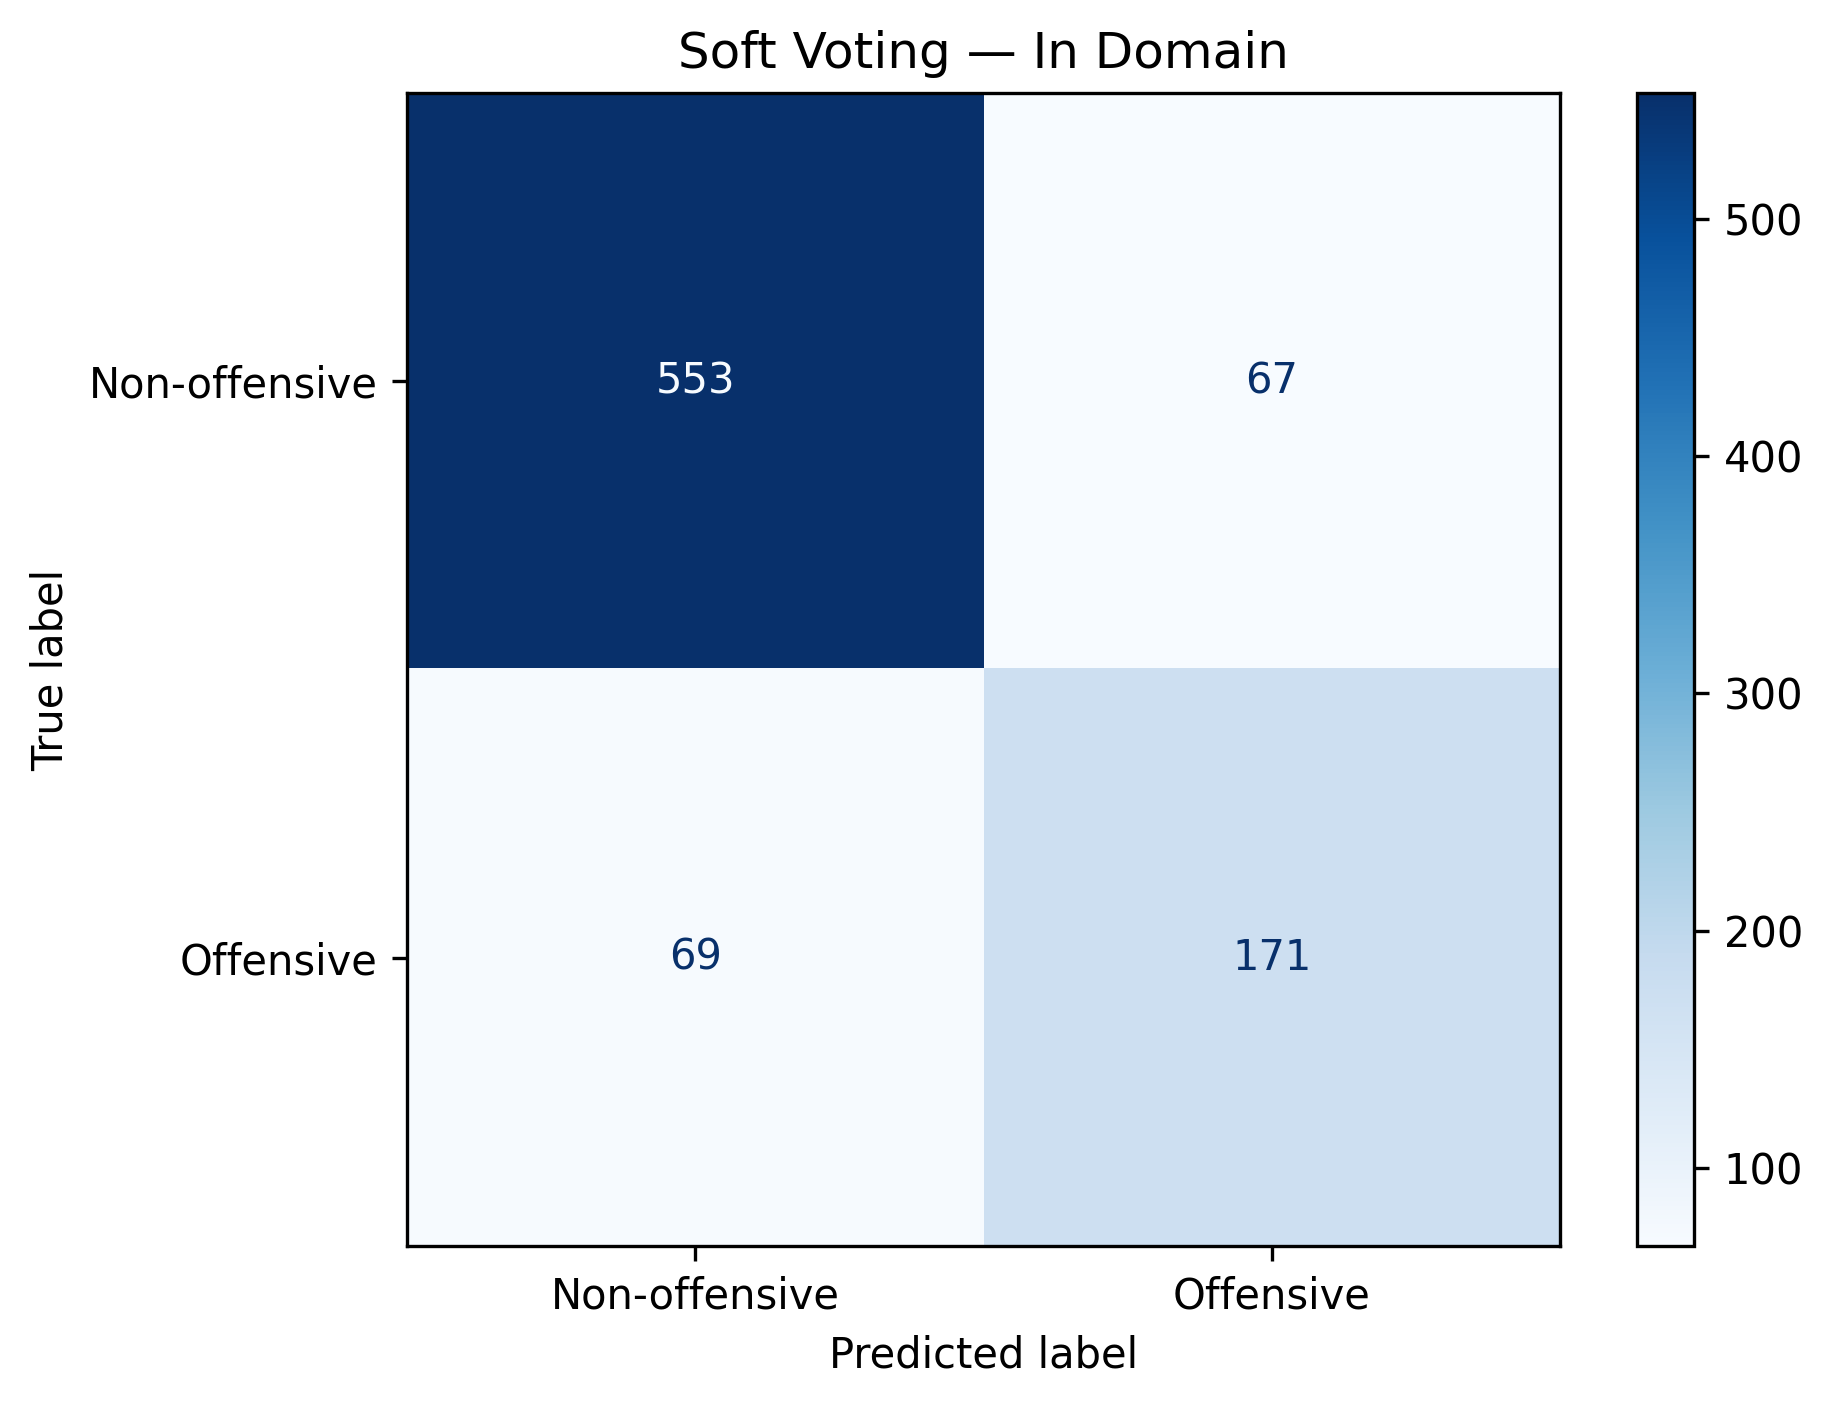
\includegraphics[width=0.44\textwidth]
{confusion_soft_voting_in_domain.png}
\hfill
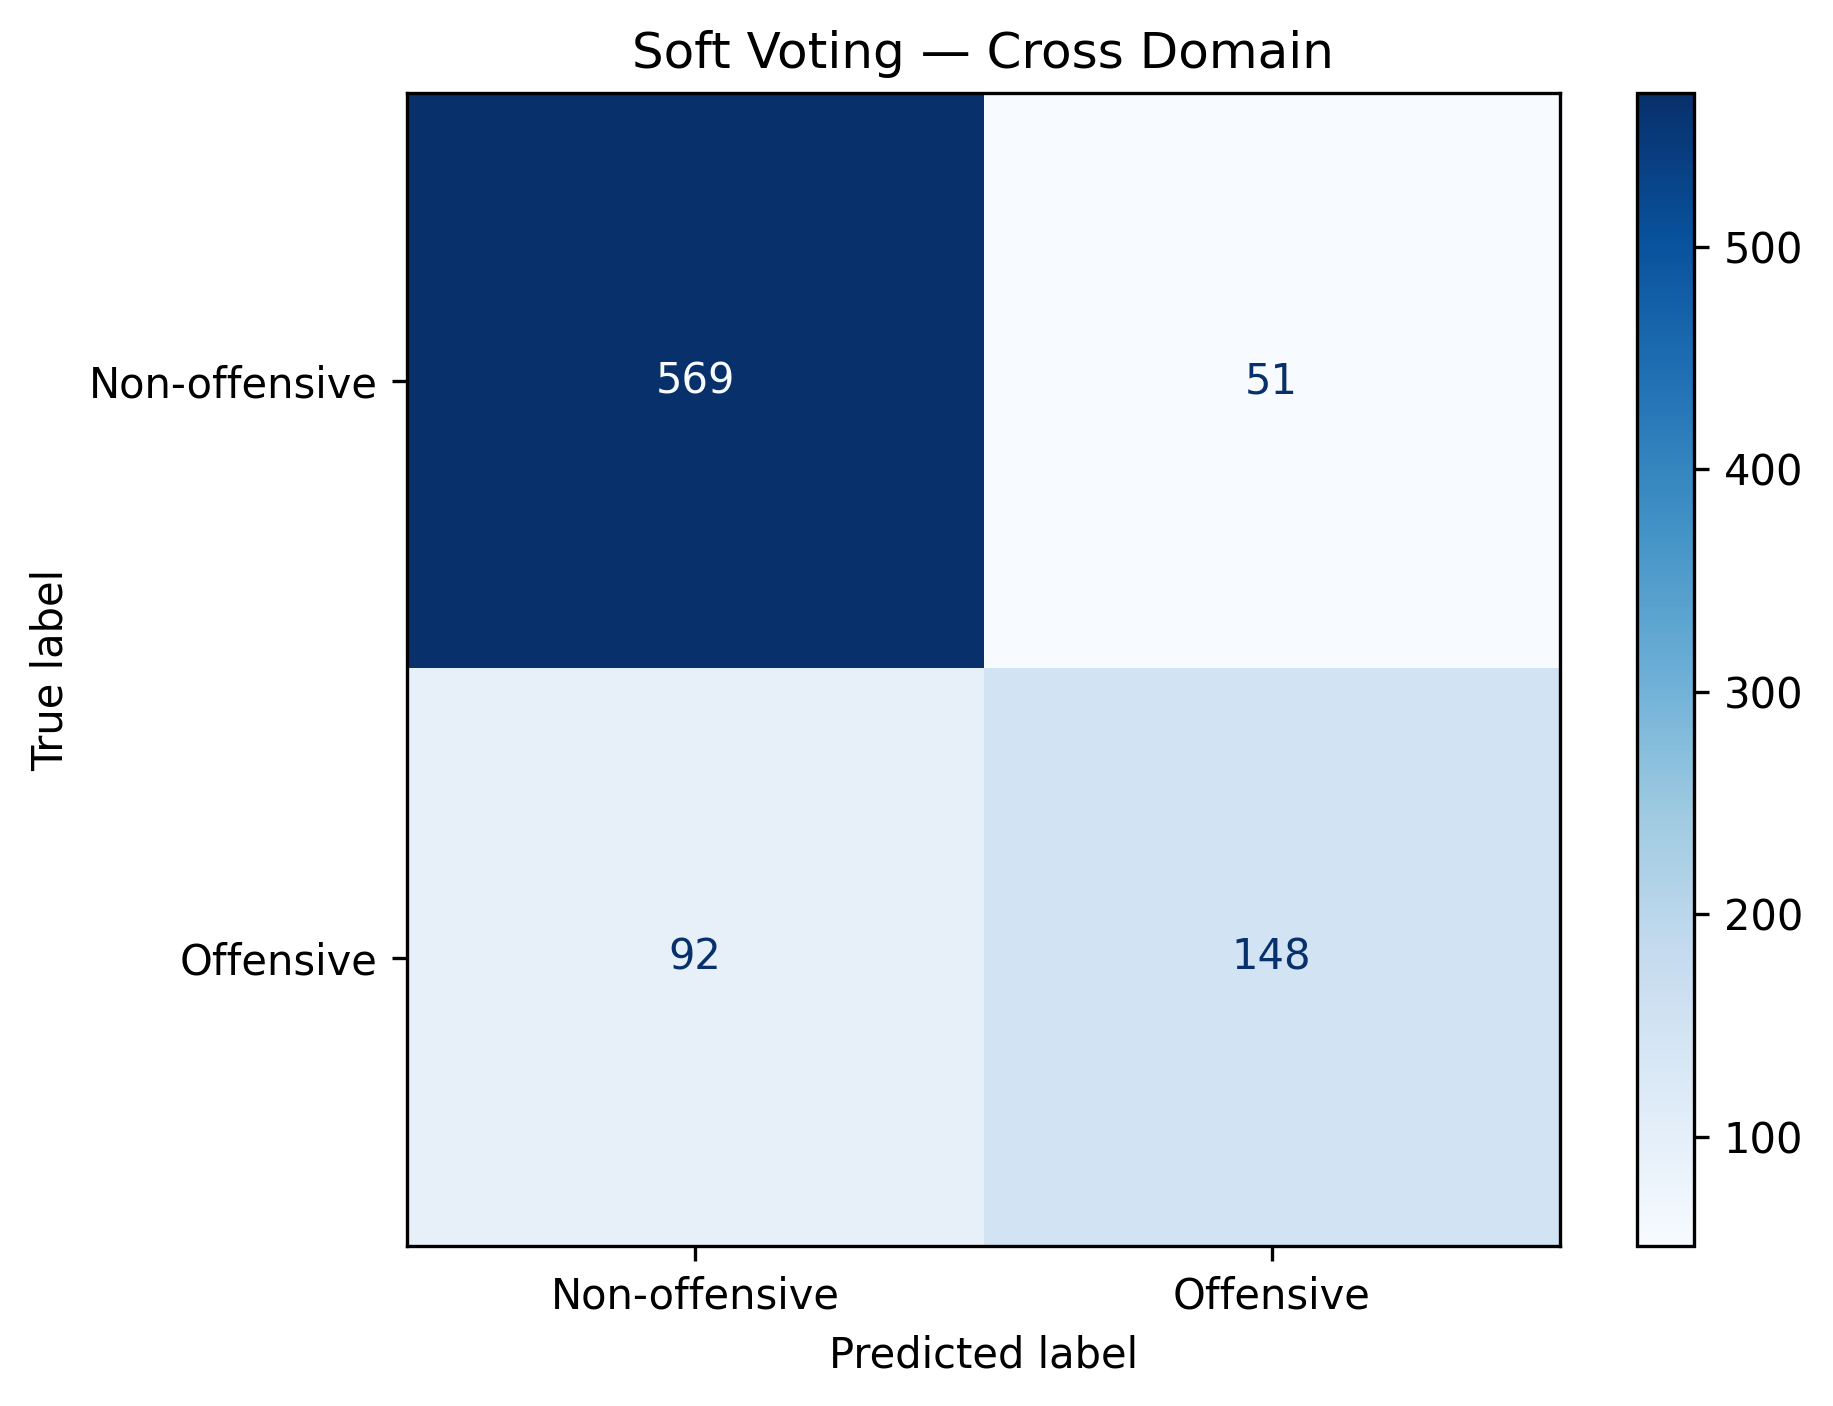
\includegraphics[width=0.44\textwidth]
{confusion_soft_voting_cross_domain.png}
\caption{Confusion matrices for soft majority voting:
in-domain (left) and cross-domain (right).}
\label{fig:soft-voting-cm}
\end{figure}

\subsection{Analysis}

In the in-domain setting, soft voting achieved an accuracy of 0.8419 and a macro-F1 score of 0.8030. Its accuracy was slightly higher than that of the individual models, while its macro-F1 was slightly lower than fBERT (0.8033).

In the cross-domain setting, soft voting achieved an accuracy of 0.8337 and a macro-F1 score of 0.7813.
This was better than BERT (0.7222) and HateBERT (0.7536) in terms of macro-F1, but lower than fBERT (0.8088).

The macro-F1 score decreased by 0.0217 between the two settings. The main difference was in the offensive class.
Its recall dropped from 0.7125 to 0.6167, while the non-offensive F1 remained relatively stable. The confusion matrices also show an increase in false negatives from 69 to 92, meaning that more offensive examples were classified as non-offensive in the cross-domain setting.

One possible reason is that the three models perform differently across domains. In the cross-domain setting, fBERT performed better than BERT and HateBERT. Since soft voting assigns equal weights to all three models, this may help explain why the ensemble did not outperform fBERT alone.

\end{document}
